\section{Toro}
\emph{Toro} has a complicated kinematic structure as shown in Figure \ref{fig:toro_kin}. It consists of 3 kinematic chains branching from the common base. The hip acts as the commnon base. The three chains branching from the hip are  upper body, right leg and left leg. The upper body further branches into right hand and left hand. The two arms and legs acts as the end effectors of \emph{Toro}.

\begin{figure}
\begin{center}
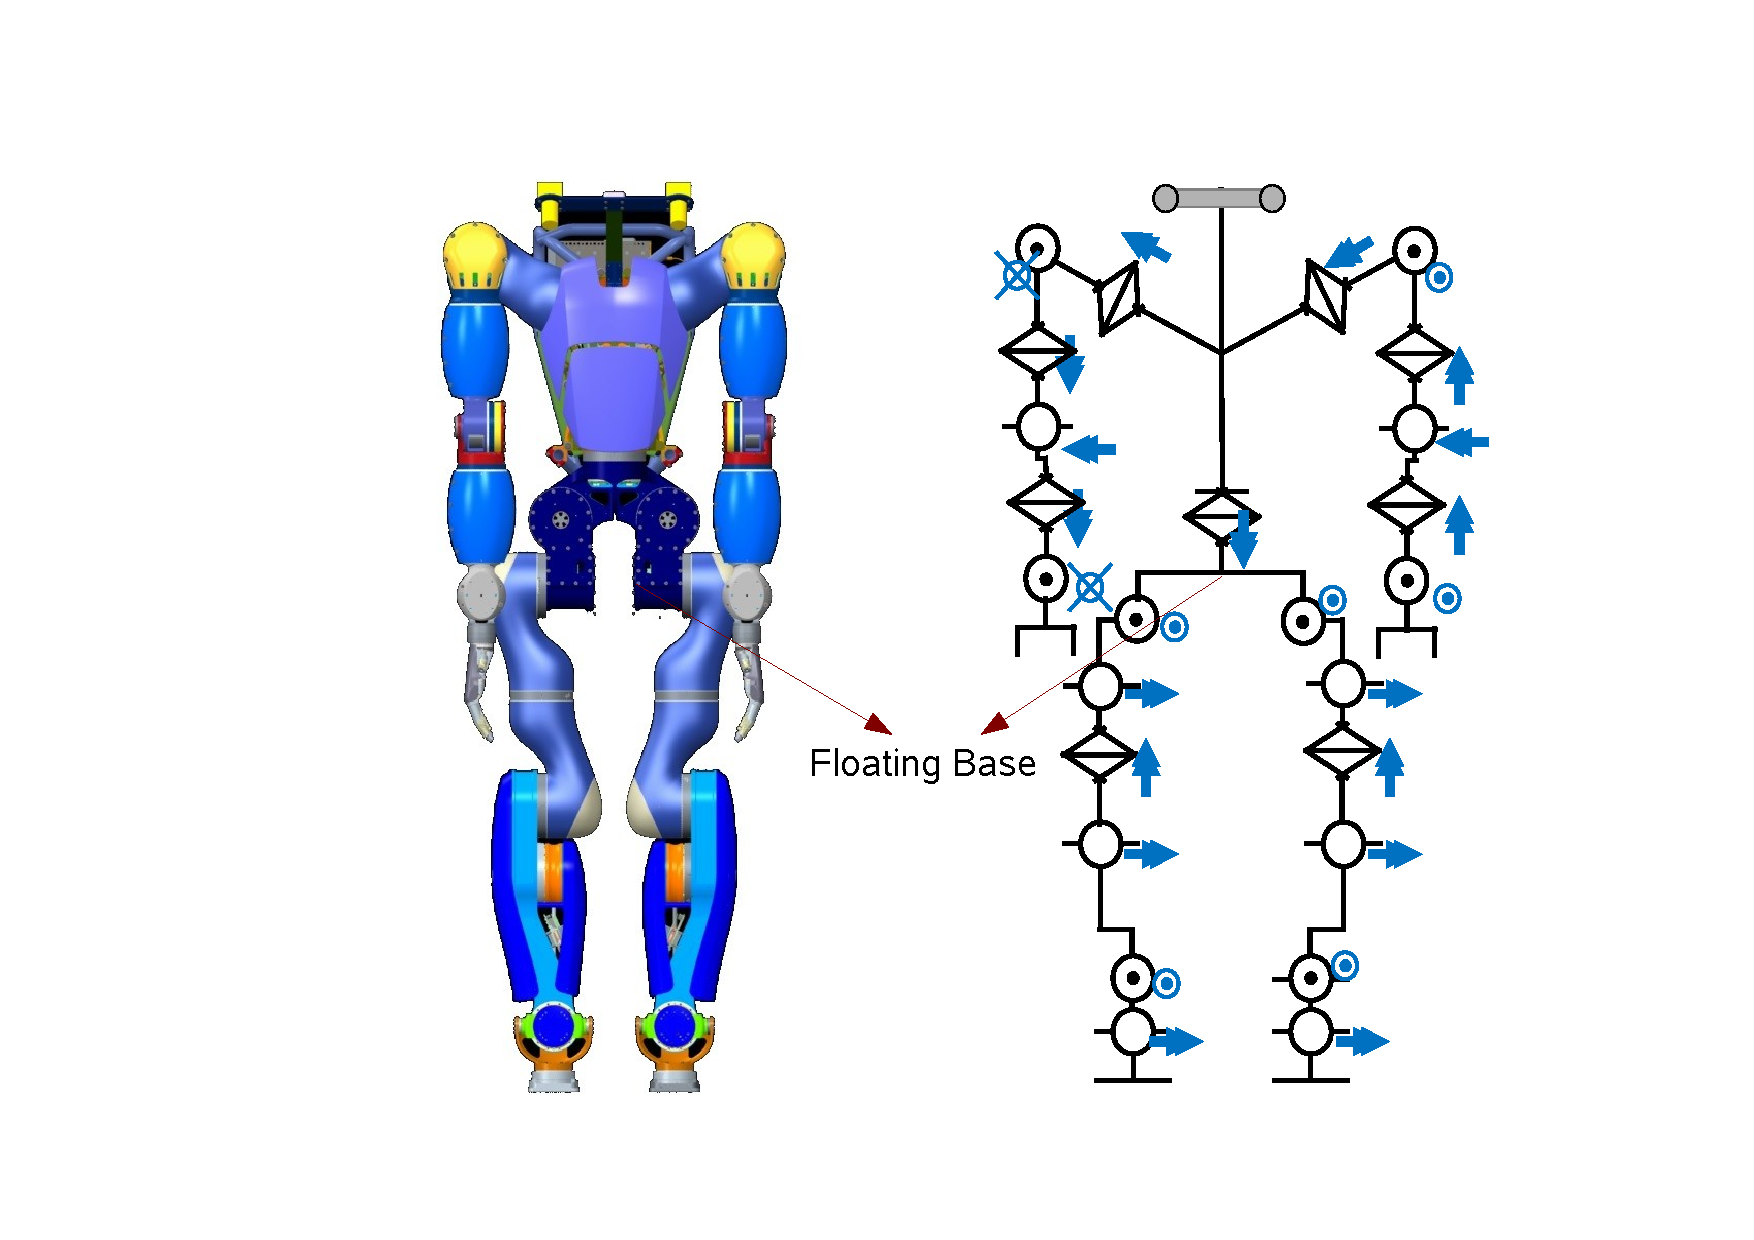
\includegraphics[trim= 70mm 10mm 40mm 10mm,clip,scale=0.7]{Bilder/TORO_kinematic.pdf}
\caption{Kinematic chain of \emph{Toro} \underline{Explain the joints symbols}}
\label{fig:toro_kin}
\end{center}
\end{figure}

The generalized coordinates of \emph{Toro} are represneted by a vector of joint angles $q$ and the coordinates of the base of robot $x^b$. Number of joints of a robot is the number of controllable degrees of freedom \cite[Chapter 2]{mur94}. The coordinates of the base $x^b$ are the underactuated degrees of freedom of \emph{Toro}. 

A rigid body in space has six degrees of freedom as shown in Figure \ref{fig:rbody}.
%\begin{figure}
\begin{figure}
\begin{center}
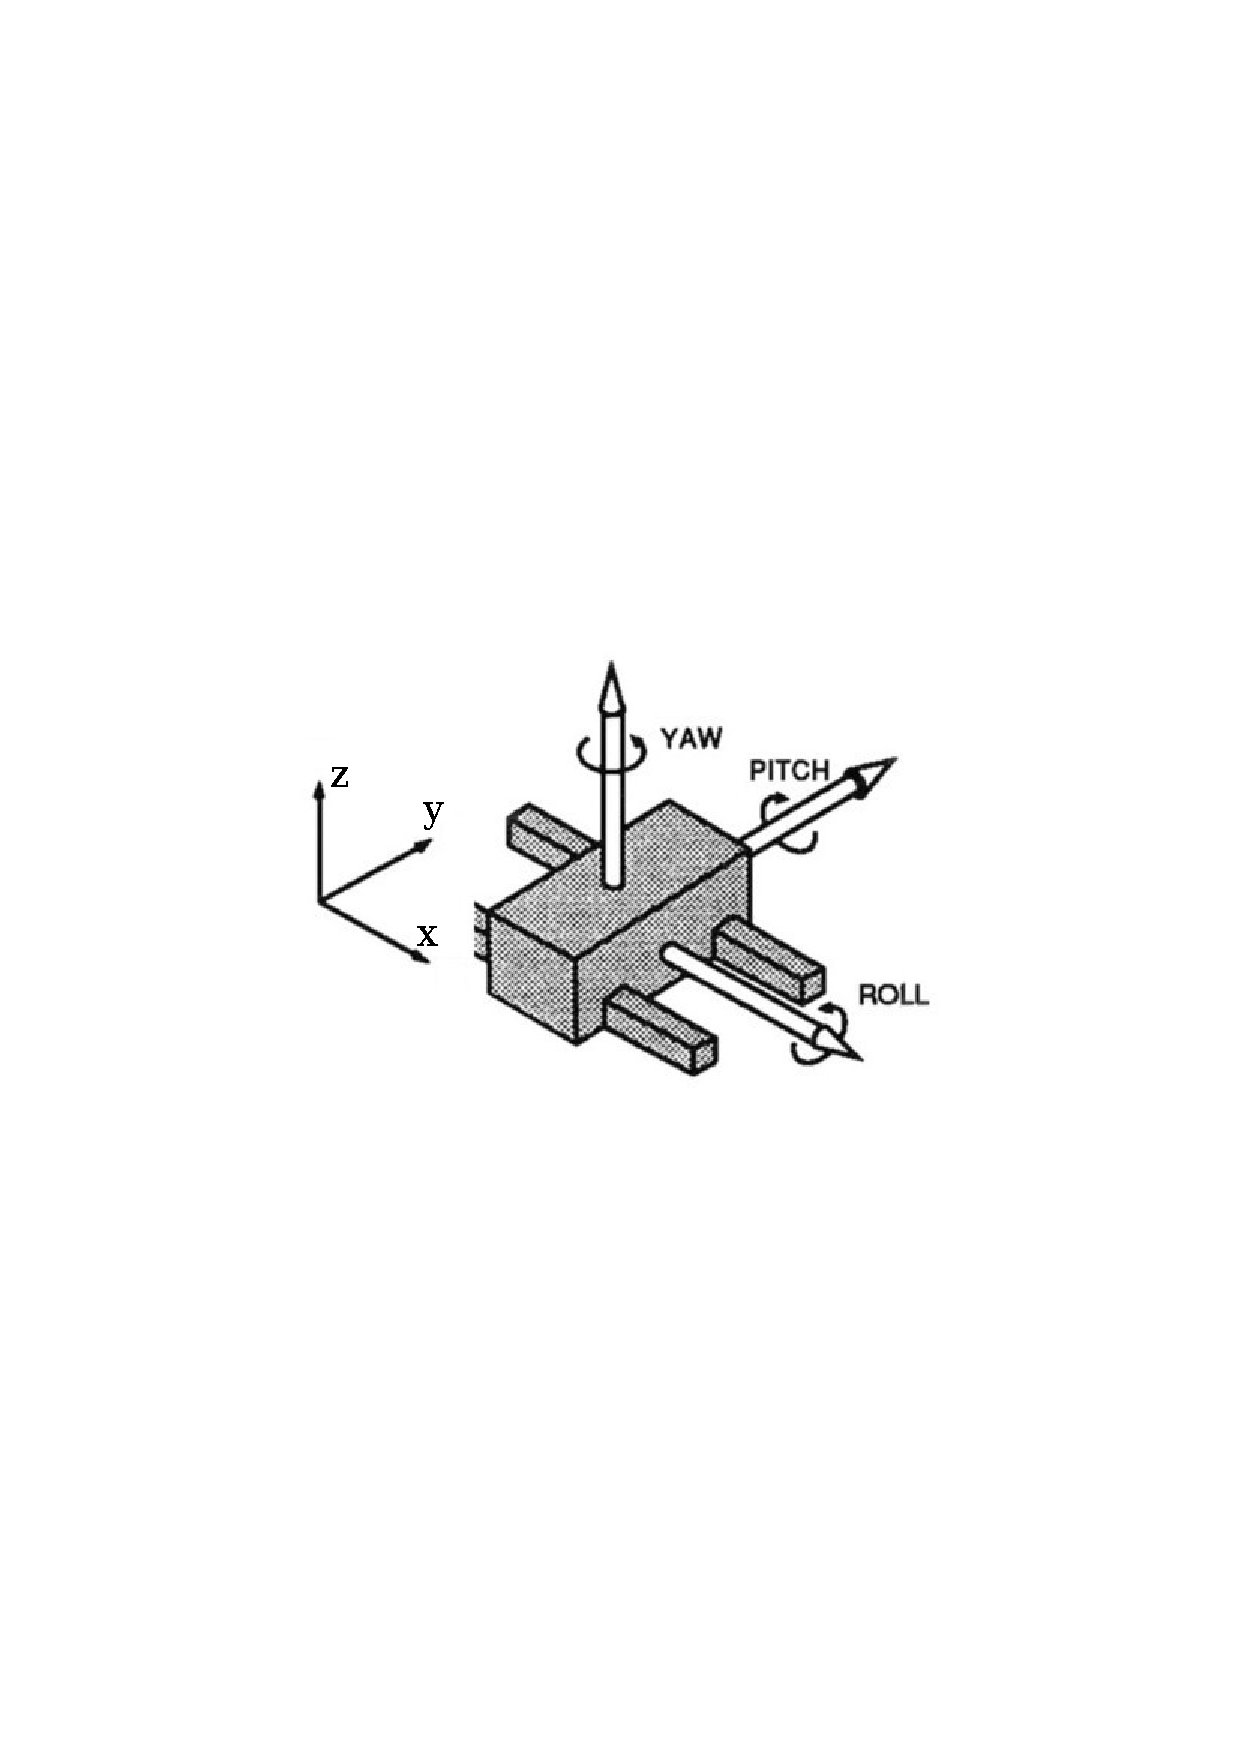
\includegraphics[trim= 30mm 100mm 10mm 120mm,scale=0.75]{Bilder/rbody_dof.pdf}
\caption[Degrees of freedom of a rigid body]{Degrees of freedom of a rigid body \footnotemark[1]}
\label{fig:rbody}
\end{center}
\end{figure}
The translational and rotational degrees of freedom of the rigid body in Figure \ref{fig:rbody} are \emph{x,y,z} and \emph{roll,pitch,yaw}. The rotational degrees of freedom \emph{roll,pitch,yaw} corresponds to rotation of the body around \textbf{X,Y,Z} axes. The base of \emph{Toro} is assumed to be a free rigid body. Since the base has all the six degrees of freedom which corresponds to degrees of freedom of rigid body floating in three dimensional space, it is called floating base. The equation of motion of a single rigid body(floating base) is given by Newton-Euler equation of motion in body coordinates \cite[Chapter 4]{mur94}. 
\footnotetext[1]{Image source:\url{http://www.cncexpo.com/Images/pitchyawroll.jpg}}
\begin{equation}
\label{eq:dyn_rig_bdy}
\begin{bmatrix}
mI_3 & \textbf{0}_3 \\ \textbf{0}_3 &\Im
\end{bmatrix}
\begin{bmatrix}
\dot{v}^b\\ \dot{\omega}^b
\end{bmatrix}
+ \begin{bmatrix}
\omega^b \times mv^b \\ 
\omega^b \times \Im w^b
\end{bmatrix}
= W^b.\\
\end{equation}
In the above equation, \emph{m} is the mass of the rigid body, $\Im$ is the moment of inertia of the rigid body. $I_3$ represents the $3 \times 3$ identity matrix and $ \textbf{0}_3$ represents the  $3 \times 3$ zero matrix. $[\dot{v}^b,\dot{\omega}^b]$ are the translational velocity and angular velocity represented in body coordinate frame. $W^b$ is the body wrench applied to the center of mass of body. The body wrench represents a force/moment pair acting on the body. It is represented by vector in $\Re^6$ as \citep{mur94}
$$ W^b = \begin{bmatrix} F \\ \tau \end{bmatrix}, $$ where $F \in \Re^3$ is the linear component and $\tau \in \Re^3$ is the rotational component of the genaralized force.

To be consistent with the multibody system dynamics formulation in Equation \ref{eq:dyn_mul_bdy} Newton Euler Equation \ref{eq:dyn_rig_bdy} is reformulated as
\begin{equation}
\label{eq:dyn_rig_bdy_sh}
M_x^b \dot V^b + C_x^b V^b+g_x^b = W^b,
\end{equation}
 where $x^b=\begin{bmatrix}p \\ \theta\end{bmatrix} \in \Re^6$ is a vector representing the position and orientation of the rigid body with respect to world coordinate frame or spatial frame. The three dimensional position vector is $p=\begin{bmatrix}p_x \\ p_y \\ p_z \end{bmatrix} \in \Re^3$ and the three dimesional orientation vector is $ \theta= \begin{bmatrix} \theta_{x} \\ \theta_{y} \\ \theta_{z} \end{bmatrix} \in \Re^3$. The orientation of the rigid body is parmeterised by Euler angles [Appendix \ref{eq:rot_full}]. 
 The body velocity $V^b$ is 
 \begin{equation}
\label{eq:body_vel}
V^b =
\begin{bmatrix}
v^b \\ \omega^b
\end{bmatrix}
= \begin{bmatrix}
R^T \dot{p} \\ (R^T \dot{R})^\vee
\end{bmatrix},
\end{equation}
where $\vee$ operator denotes the extraction of 3 dimensional vector from a skew symmetric matrix[Appendix \ref{sec:avel_trfm}]. The rotation matrix $R$ is the matrix dependent on parameterization of Euler angles [Appendix \ref{eq:rot_full}]. The acceleration $\dot{V}^b$ is the acceleration with respect to body frame. $M_x^b$ represents the inertia matrix of the rigid body in body coordinates. $C_x^b$ is the matrix representing the Coriolis and centrifugal forces acting on the system in body coordinates. $g_x^b$ is the vector representing the gravitational forces acting on the body in body coordinates. $W^b$ is the external force applied to the center of mass of the body. \footnote[2]{Inertia, Coriolis and gravity are assumed to be given with respect to the body coordinate frame for the rest of the report}.

The equations of motion of \emph{Toro} in Figure \ref{fig:toro_kin} is composed of equation of motion of the multibody system and equation of motion of single rigid body. The equation of motion of \emph{Toro} is formulated like the equation of motion for a floating base system as given in \cite{ott09}.
\begin{equation} \label{eq:dyn_biped}
\begin{bmatrix}
M_x &M_{xq} \\ M_{qx} &M_q
\end{bmatrix}
\begin{bmatrix}
\ddot{x}^b \\ \ddot{q}
\end{bmatrix}
+
\begin{bmatrix}
C_x &C_{xq} \\ C_{qx} &C_q
\end{bmatrix}
\begin{bmatrix}
\dot{x}^b \\ \dot{q}
\end{bmatrix}
+
\begin{bmatrix}
g_x \\ g_q
\end{bmatrix}
=
\begin{bmatrix}
0 \\ \tau
\end{bmatrix}
+ (J_r^b)^T W_r^b + (J_l^b)^T W_l^b,
\end{equation}
where the terms with subscript $x$ are the parameters of floating  base, the terms with subscript $q$ are the parameters of the multibody system and the terms with subscript $xq, qx$ are the coupling terms that connects the dynamics of the floating base with dynamics of the multibody system.

Equation \ref{eq:dyn_biped} can be written in a simplified form as
\begin{equation} \label{eq:dyn_sbiped}
M(y)\ddot{y} + C(y,\dot{y})\dot{y} + g(y) = \tau + (J_r^b)^T W_r^b + (J_l^b)^T W_l^b,
\end{equation}
where $y = \begin{bmatrix} x^b \\ q \end{bmatrix}$ is the vector representing the state variables of \emph{Toro}. The generalized coordinates of multibody system is $q \in \Re^{25}$ which represents the vector of joint angles. The vector of generalized velocities is $\dot{y}=\begin{bmatrix} V^{b} \\ \dot{q} \end{bmatrix} \in \Re^{31}.$ The vector of generalized accelerations is $\ddot{y}\in \Re^{31}.$  $M(y)\in \Re^{31 \times 31}$ is the inertia matrix, $C(y,\dot{y})\in \Re^{31 \times 31}$ is the matrix accounting for centrifugal and Coriolis forces. $g(y) \in \Re^{31}$ is the gravity vector. $\tau \in \Re^{31}$ is the vector of actuating torques acting on the robot, where the first six components are zero because those degrees of freedom corresponding to $x_f$ are not actuated. $J_r^b,J_l^b \in \Re^{31 \times 6}$ are the body Jacobian matrices that transforms the wrenches $W_r^b,W_l^b \in \Re^{6}$ applied in the right and left foot to generalized forces acting on the robot. From here on the super script $b$ in body Jacobian matrix and body wrenches is omitted for the sake of simplicity.

The forward dynamics equation of \emph{Toro} is
\begin{equation}
	\label{eq:motion}
	\ddot{y} = M(y)^{-1}(-C(y,\dot{y})\dot{y} - g(y) + J_r(y)^{T}W_{r} +J_l(y)^{T}W_{l} + \tau). 
\end{equation}

\subsection{State space representation:}
The state space representation of \emph{Toro} is formulated similar to the state space representation of multibody system in Equation \ref{eq:dyn_ss}.
\begin{equation}
\label{eq:newton_motion}
 \begin{bmatrix}
\dot{pos} \\ \dot{vel}
\end{bmatrix}
= \begin{bmatrix}
vel \\ acc
\end{bmatrix}
\end{equation}
acceleration(\emph{acc}) is given by the forward dynamics of the system.

The equations of motion in Equation \ref{eq:motion} should be formulated in state space form of nonlinear systems as given in \ref{eqn:nl_sys}.
\begin{comment}
General state space representation of a nonlinear system
\begin{equation}
\label{eq:dyn_nl}
	\begin{split}
	\dot{x} = f(x,u)\\
	y = h(x,u)
	\end{split}
\end{equation}
where, $x \in \Re^{n}$ is the vector representing the states of the system. $u \in \Re^{p}$ is the vector of inputs acting on the system. $y \in \Re^{m}$ is the vector of outputs of the system.\\
\end{comment}
 \emph{R} is the rotation matrix which describes the rotation of rigid body with respect to \underline{spatial frame}. It is possible to reformulate the translational velocity of the above equation in first order \underline{ODE(Ordinary Differential Equation)}. It is not straight forward to obtain the time rate of change of Euler angles $\dot{\theta}$. There exists a transformation between the $\dot{\theta}$ and angular velocity $\omega^b$.
\begin{equation}
\label{eq:transfo_angvel}
\begin{split}
\omega^b = T(\theta)\dot{\theta}
\end{split}
\end{equation}
$T(\theta)$ is the transformation matrix [Appendix \ref{sec:avel_trfm}]. 

The state space representation of the equation of motions of \emph{Toro} can be obtained by substituting Equations \ref{eq:body_vel}, \ref{eq:transfo_angvel} and \ref{eq:motion} in Equation \ref{eq:newton_motion}

\begin{equation}
\label{eq:toro}
	\dot{x} = 
	\begin{bmatrix}
	\dot{p} \\ \dot{\theta} \\ \dot{q} \\ \ddot{y}
	\end{bmatrix}
	=
	\begin{bmatrix}
	R v^b\\	
	T(\theta)^{-1} \omega_f^b \\
	\dot{q}\\
	M(y)^{-1}(-C(y,\dot{y})\dot{y} -g(y) +  J_r(y)^{T}W_{r} +J_l(y)^{T}W_{l} + \tau)	
	\end{bmatrix}
	\\
	\end{equation}	
\begin{itemize}
\item $$ y = \begin{bmatrix} p \\ \theta \\ q \end{bmatrix} = \begin{bmatrix} x_f \\ q \end{bmatrix}, \dot{y} = \begin{bmatrix} V^b \\ \dot{q}\end{bmatrix}, x = \begin{bmatrix}y \\ \dot{y}\end{bmatrix} $$  $x_f,q$ are the parameters of the floating base and joints as described in \ref{eq:motion}. $V^b$ is the body velocity as defined in \ref{eq:body_vel} and $\dot{q}$ is the velocities of the joints of the robot. \emph{x} is the vector of system states.
\item $T(\theta_{f})$ is the matrix that transforms the angular velocity $\omega_{f}^{b}$ to the time derivative of Euler angles $\dot{\theta}_{f}$. i.e $\omega_{f}^{b}=T(\theta_{f}) \dot{\theta}_{f}$. 
\item R is the rotation matrix which describes the rotation of floating base with respect to spatial frame. $ R = R_x(\theta_x) R_y(\theta_y) R_z(\theta_z)$
\end{itemize}

\section{Prediction step}
The prediction equations of EKF are given in Equation \ref{eq:ekf_predict}. For the sake of simplicity we assume the process noise acting on the model is uncorrelated. i.e The noise acting on each state is independent $$W_k = I_{n}$$. \emph{n} is the number of states. Substituting the value of $W_k$ in Equation \ref{eq:ekf_predict}
\begin{equation}
\label{eq:predict}
\begin{split}
\hat{x}_{k+1}^- &= f(\hat{x}_{k},u_{k+1},0)\\
P_{k+1}^- &= A_kP_{k}A_k^T + Q_{k}\\
\end{split}
\end{equation}
The model is discretized for the implementation of EKF. Since the time step for integration is very small $\Delta t = 1ms$ forward Euler discretization method is used to discretize the continuous time model in \ref{eq:toro}.
\begin{equation}
\label{eq:toro_dis}
	\begin{bmatrix}
	\hat{p}_{k+1}^- \\ \hat{\theta}_{k+1}^- \\ \hat{q}_{k+1}^- \\ \hat{\dot{y}}_{k+1}^-
	\end{bmatrix}
	 =   
	 \begin{bmatrix}
	 \hat{p}_k \\ \hat{\theta}_k \\ \hat{q}_k \\ \hat{\dot{y}}_{k}
	\end{bmatrix}	  
	+ \Delta t f(\hat{x}_k,u_{k+1}) \\
\end{equation}
$$ f(\hat{x}_k,u_{k+1}) = 
	\begin{bmatrix}
	R v^b_k\\	
	T(\hat{\theta}_k)^{-1} \omega_k^b\\
	\dot{q_k}\\
	M(\hat{y}_{k})^{-1}(-C(\hat{y}_{k},\hat{\dot{y}}_{k})\hat{\dot{y}}_{k} -g(\hat{y}_{k}) +  J_r(\hat{y}_{k})^{T}W_{r,k+1} +J_l(\hat{y}_{k})^{T}W_{l,k+1} + \tau_{k+1})	
	\end{bmatrix} $$
$\hat{x}(t_k) = \hat{x}(k \Delta t) = \hat{x}_k$ represents the state x at \emph{kth} sampling instant. $\hat{x}_{k+1} = \hat{x}(k \Delta t + \Delta t)$ represents the state of the system at the next sampling instant. $u_{k+1}$ is the input at sampling instant $k+1$. It is assumed that the value of the input remains constant in the interval between two sampling instant. This assumption is valid because of the zero order hold mechanism in sensor circuitry.

Equation \ref{eq:toro_dis} is used to predict the state $\hat{x}_k$ in Equation \ref{eq:predict}. For the computation of state covariance matrix $P_k^-$ in Equation \ref{eq:predict}, the \underline{Jacobian Matrix} is computed for Equation \ref{eq:toro_dis}. \underline{The Jacobian} computation of the different parts of the equation is follows,
From Equation \ref{eq:toro_dis}
\begin{enumerate}
\item $ \hat{p}_{k+1}^- = \hat{p}_k + \Delta t Rv_b$, $ \hat{p}_k = [\hat{p}_{x,k},\hat{p}_{y,k},\hat{p}_{z,k}]$
\begin{equation}
\label{eq:dpdx}
\dfdx{\hat{p}_{j,k+1}^-}{x} = \left(\dfdx{\hat{p}_{j,k+1}^-}{x_{1}}, \dfdx{\hat{p}_{j,k+1}^-}{x_{2}}, \cdots , \dfdx{\hat{p}_{j,k+1}^-}{x_{62}}\right) \in \Re^{3 \times 62}
\end{equation}
\[
 \dfdx{\hat{p}_{k+1}^-}{x_{i}} =  \left\lbrace
  \!\begin{aligned}
   &e_i & \text{if }(i=j)\\
   &\Delta t \dfdx{R}{x_i}v_b & \text{if }(3 < i \leq 6)\\
   &\textbf{0}_{3 \times 1} &\text{if}(6 < i \leq 31) \text{ or } (35 < i \leq 62) \\
   &col(R,i-31) & \text{if } 31 < i \leq 34 \\
  \end{aligned} \right.
\]
\begin{itemize}
\item \emph{j} in the subscript represents the row dimension and  \emph{i} represents the column dimension of the matrix in Equation \ref{eq:dpdx}
\item $col(X,i)$ - represents the \emph{ith} column of matrix $X$.
\item $\dfdx{R}{x_i}$ is the partial derivative of \emph{R} with respect to the state $\hat{x}_k$ (i.e euler angles [Appendix \ref{sec:rot_mat}]), $e_i$ is the unit vectors in direction of coordinate axis and  $\textbf{0}_{3 \times 1}$ is the zero vector of dimensions $3 \times 1$ [Appendix \ref{sec:symbols}].
\end{itemize}

\item $\hat{\theta}_{k+1}^- = \hat{\theta}_k + \Delta t T(\hat{\theta}_k)^{-1} \omega_k^b$
\begin{equation}
\label{eq:dthetadx}
\dfdx{\hat{\theta}_{j,k+1}^-}{x} = \left(\dfdx{\hat{\theta}_{j,k+1}^-}{x_{1}}, \dfdx{\hat{\theta}_{j,k+1}^-}{x_{2}}, \cdots , \dfdx{\hat{\theta}_{j,k+1}^-}{x_{62}}\right) \in \Re^{3 \times 62}
\end{equation}
\[
 \dfdx{\hat{\theta}_{k+1}^-}{x_{i}} = \left\lbrace
  \!\begin{aligned}
   &\textbf{0}_{3 \times 1} &\text{if}(0 < i \leq 3) \text{ or }(6 < i \leq 31) \text{ or } (35 < i \leq 62) \\
   &e_{i-3} + \Delta t \dfdx{T(\hat{\theta}_k^-)^{-1}}{x_i}\omega_k^b & \text{if}3< \text{i} \leq 6 \\
   &col(T(\hat{\theta}_k^-)^{-1},i-34) & \text{if } 31 < i \leq 34 \\
  \end{aligned} \right.
\]
\begin{itemize}
\item $\dfdx{T(\theta_k^-)^{-1}}{x_i}$ is the partial derivative of inverse of transformation matrix with respect to state [Appendix \ref{sec:avel_trfm}] 
\end{itemize}

\item $\hat{q}_{k+1}^- = \hat{q}_k + \Delta t \dot{q}_k $
\begin{equation}
\label{eq:dqdx}
\dfdx{\hat{q}_{k+1}^-}{x} = \left(\dfdx{\hat{q}_{k+1}^-}{x_{1}}, \dfdx{\hat{q}_{k+1}^-}{x_{2}}, \cdots , \dfdx{\hat{q}_{k+1}^-}{x_{62}}\right) \in \Re^{25 \times 62}
\end{equation}
\[
\dfdx{\hat{q}_{k+1}^-}{x_{i}} = 
	\begin{cases}
	l_{25,i} & \text{if } (6 < i \leq 31) \text{ or } (38 < i \leq 62) \\
	0 & \text{otherwise}   \\
	\end{cases}
\]
\begin{itemize}
\item $l_{25,i}$ is a column vector of length 25 with 1 in the \emph{ith} position and zeros in other position [Appendix \ref{sec:symbols}].
\end{itemize}
\item $\hat{\dot{y}}_{k+1}^- = \hat{\dot{y}}_{k}+ \Delta t \Lambda $
$$\Lambda = M(\hat{y}_{k})^{-1}(-C(\hat{y}_{k},\hat{\dot{y}}_{k})\hat{\dot{y}}_{k} - g(\hat{y}_{k}) + J_r(\hat{y}_{k})^{T}W_{r,k+1} +J_l(\hat{y}_{k})^{T}W_{l,k+1} + \tau_{k+1})$$
 \begin{equation}
 \label{eq:dydx}
\dfdx{\hat{\dot{y}}_{k+1}^-}{x} = \left(\dfdx{\hat{\dot{y}}_{k+1}^-}{x_{1}}, \dfdx{\hat{\dot{y}}_{k+1}^-}{x_{2}}, \cdots , \dfdx{\hat{\dot{y}}_{k+1}^-}{x_{62}}\right) \in \Re^{31 \times 62}
\end{equation}
where,
\[
\dfdx{\hat{\dot{y}}_{k+1}^-}{x_{i}} = 
\left\{ 
\!\begin{aligned}
	& \left. \!\begin{aligned}
	-M_k^{-1}\dfdx{M_k}{x_{i}}\Lambda + &M_k^{-1}\left(-\dfdx{C_k}{x_{i}}\hat{\dot{y}}_{k} -\dfdx{g_k}{x_{i}}        + \left(\dfdx{J_{r,k}^{b}}{x_{i}}\right)^{T}W_{r,k+1}\right) \\
	& + M_k^{-1}\left(\dfdx{J_{l,k}^{b}}{x_{i}}\right)^{T}W_{l,k+1}
	\end{aligned} \right\}& \text{if } 0 < i \leq 31 \\
&l_{31,(i-31)}-M_k^{-1}\dfdx{M_k}{x_{i}}\Lambda + M_k^{-1}\left(-\dfdx{C_k}{x_{i}}\hat{\dot{y}}_{k}- col(C_k,i-31)\right) & \text{if } i < 31  \\
\end{aligned}
\right.
\]
\begin{itemize}
\item $M_k= M(\hat{y}_{k}),C_k=C(\hat{y}_{k},\hat{\dot{y}}_k),J_{r,k}=J_r(\hat{y}_{k}),J_{l,k}=J_l(\hat{y}_{k})$
\end{itemize}
The system matrix $A_k$ in Equation \ref{eq:predict} is formulated by combining Equations \ref{eq:dpdx},\ref{eq:dthetadx},\ref{eq:dqdx} and \ref{eq:dydx}
\begin{equation}
\label{eq:sys_mat}
A_k = \left(
\begin{aligned}
\dfdx{\hat{p}_{k+1}^-}{x} \\
\dfdx{\hat{\theta}_{k+1}^-}{x} \\
\dfdx{\hat{q}_{k+1}^-}{x}\\
\dfdx{\hat{\dot{y}}_{k+1}^-}{x}
\end{aligned} \right)
\in \Re^{62 \times 62}
\end{equation}
Substituting Equations \ref{eq:toro_dis} and \ref{eq:sys_mat} in \ref{eq:predict} and substituting the values of process covariance $Q_k$ completes the prediction stage of EKF.

\section{Update step}
The update equation of the EKF is given in Equation \ref{eq:ekf_correct}. The measurement equation of the system is given by $$\hat{y}_{k+1} = h(\hat{x}_{k+1}^-,u_{k+1},0)$$.For the sake of simplicity let us assume the measurement of noise are independent. $$V_k = I_3$$. Substituting the assumption in \ref{eq:ekf_correct}
\begin{equation}
\label{eq:correct}
\begin{split}
K_{k+1} &= P_{k+1}^-\hat{H}_{k+1}^{T-}(\hat{H}_{k+1}^-P_{k+1}^-\hat{H}_{k+1}^{T-} + R_{k+1})^{-1}\\
\hat{x}_{k+1} &= \hat{x}_{k+1}^- + K_{k+1}(y_{k+1}-\hat{y}_{k+1})\\
P_{k+1} &= (I- K_{k+1}\hat{H}_{k+1}^-)P_{k+1}^-
\end{split}
\end{equation}
The measurements of \emph{Toro} are Cartesian accelerations($acc^b$) of the hip measured by accelerometer($IMU_{acc}$), angular velocity($\omega^b$) of the hip measured by the gyroscope($IMU_{gyro}$), joint angles($q_j$) and joint velocities($\dot{q_j}$) measured by joint encoders.
\begin{equation}
    \label{eq:y_sens}
     y_{sens} = \begin{bmatrix} acc^b \\ \omega^b \\ q_j \\ \dot{q}_j \end{bmatrix} 
\end{equation}
\begin{itemize}
    \item The simplified model of $IMU_{acc}$ is $$ acc^b= \begin{bmatrix} acc^b_x \\ acc^b_y \\ acc^b_z \end{bmatrix} =  \begin{bmatrix}\ddot{p}_x^b \\ \ddot{p}_y^b \\ \ddot{p}_z^b \end{bmatrix} - R^T \begin{bmatrix}0 \\0 \\-9.81 \end{bmatrix}$$ \emph{R} is the rotational matrix that transforms a vector in body coordinate frame to spatial frame.
    \item $\ddot{p}^b$ is computed from the forward dynamic equation \ref{eq:motion} using the predicted values of the state
    \item $\omega_{f}^{b} $ is the vector of angular rates of the hip(floating base) measured by gyroscope. The measurements are in the frame attached to the hip. 
\end{itemize}
\begin{figure}
    \begin{center}
    %trim option's parameter order: left bottom right top
    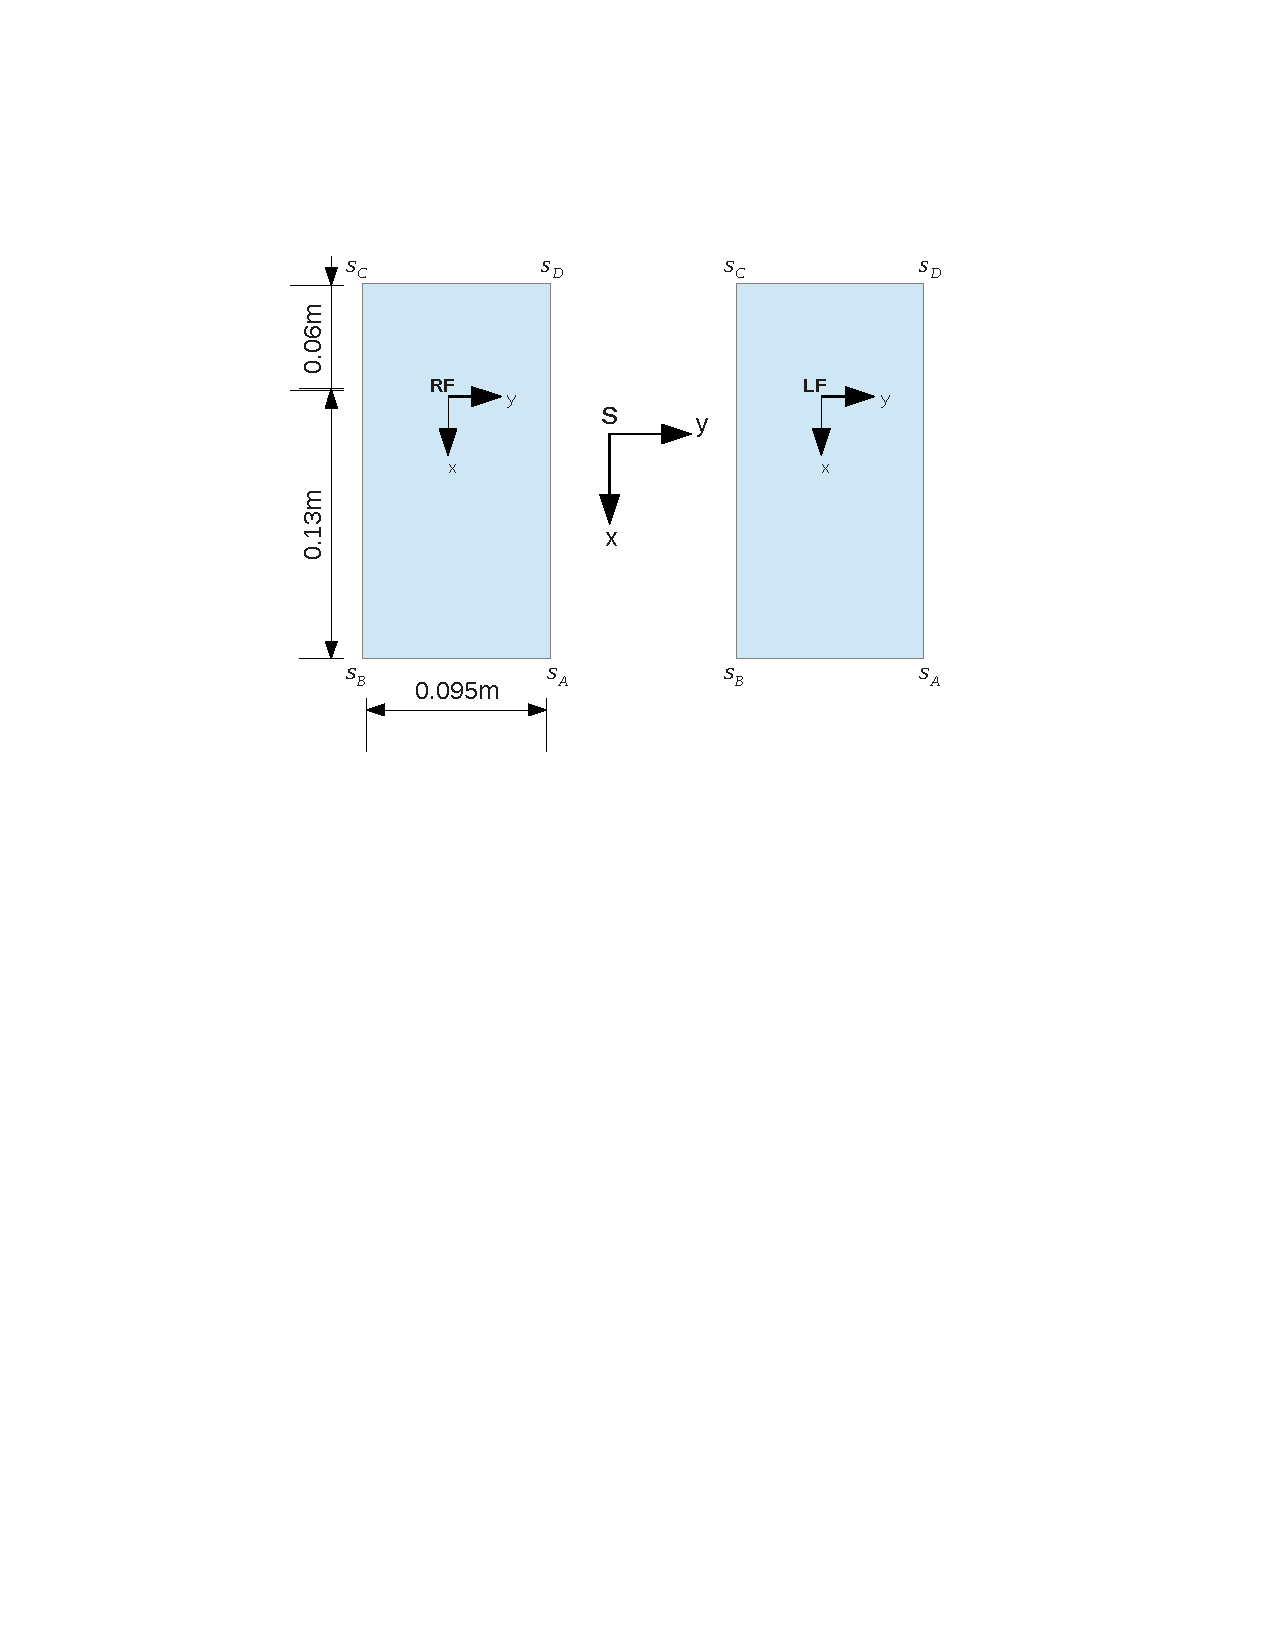
\includegraphics[trim= 20mm 150mm 20mm 50mm,scale=0.80]{Bilder/foot_topview.pdf}
    \caption{Toro feet viewed from top}
    \label{fig:biped_feet}
    \end{center}
\end{figure}
Along with the sensor measurements kinematic constraints are also considered as mesurement. When a foot is in contact with the ground the velocity of the foot is zero. Figure \ref{fig:biped_feet} shows the contact points considered for measurements. The corner points of each foot are measured with respect to spatial frame \emph{S} as shown in Figure \ref{fig:biped_feet} before starting the experiment and they are assumed to be constant throughout the experiment. The contact points of the robot does not change throughout the experiment, since we are considering the case where the robot is tilting around one edge of the foot. 
\begin{equation}
    \label{eq:y_kin}
    \begin{split}
    y_{kin} &=
    \begin{bmatrix}
    p_{contact} \\ V_{contact}
    \end{bmatrix}\\
    p_{contact} &= \begin{bmatrix}p_{RF}\\ p_{LF}\end{bmatrix}\\
     V_{contact} &= \begin{bmatrix} V_{RF}^b \\ V_{LF}^b \end{bmatrix} = \begin{bmatrix} J_r(\hat{y})^T \hat{\dot{y}} \\ J_l(\hat{y})^T\hat{\dot{y}} \end{bmatrix}
    \end{split}
\end{equation}
\begin{itemize}
\item $p_{RF},p_{LF}$ are the vectors of contact points in right foot and left foot defined with respect to spatial frame.
\item $J_r(y), J_l(y)$ are the Jacobian of right and left foot that relates the joint velocity to the velocity of right and left foot respectively. \underline{[Appendix Define Body Jacobian]}
\end{itemize}
\begin{equation}
    \begin{split}
    p_{RF} &= \begin{bmatrix} p_{A,RF}\\ p_{B,RF}\\ p_{C,RF}\\ p_{D,RF}\end{bmatrix}= \begin{bmatrix} {H}_{RF}p_{A}\\  {H}_{RF}p_{B}\\  {H}_{RF}p_{C}\\  {H}_{RF}p_{D}\end{bmatrix} \\
    p_{LF} &= \begin{bmatrix} p_{A,LF}\\ p_{B,LF}\\ p_{C,LF}\\ p_{D,LF}\end{bmatrix}= \begin{bmatrix} {H}_{LF}p_{A}\\  {H}_{LF}p_{B}\\  {H}_{LF}p_{C}\\  {H}_{LF}p_{D}\end{bmatrix} \\
    \end{split}
\end{equation}
\begin{itemize}
\item $\hat{H}_{RF},\hat{H}_{LF}$ are the homogeneous transformation matrices of the right and left foot [Appendix \ref{sec:htm}]
\item In Figure \ref{fig:biped_feet} $p_A,p_B,p_C,p_D$ are the corner points defined with respect to respective foot frame \emph{RF,LF}.
\end{itemize}
The full measurement equations of is obtained combining Equations \ref{eq:y_sens} and \ref{eq:y_kin} 
\begin{equation}
    \label{eq:y_msr}
    y_{k+1} = \begin{bmatrix} y_{sens,k+1} \\ y_{kin,k+1} \end{bmatrix}
\end{equation}
The measurement sensitivity matrix can be computed by taking the parial derivative of the measurement equation \ref{eq:y_msr} with respect to system states \emph{x}.
\begin{enumerate}
\item $\hat{acc}^b_{k+1} = \ddot{p}_{k+1}-\hat{R}^T\begin{bmatrix} 0 \\ 0 \\ -9,81 \end{bmatrix}$
\begin{equation}
    \label{eq:dacc_msrdx}
    \dfdx{\hat{acc}_{k+1}^{b-}}{x} = \dfdx{\hat{\ddot{p}}_{k+1}^{b-}}{x} + \dfdx{\hat{R}^{T-}_{k+1}}{x}\begin{bmatrix} 0 \\ 0 \\ -9,81 \end{bmatrix}  \in \Re^{3 \times 62}
\end{equation}
\begin{itemize}
    \item $\dfdx{\hat{\ddot{p}}_{k+1}^b}{x}$ is partial derivative of acceleration of body with respect to states of the system. It is computed by substituting $\hat{x}_{k+1}^-$ for $\hat{x}_k$ in Equation \ref{eq:dydx} and then subtracting  $l_{31,i-31}$ for the case \emph{i > 31}. The first three rows of the resulting matrix is the partial derivative of acceleration with respect to states.
    \item $\dfdx{\hat{R}^T_{k+1}}{x}$ is partial derivative of Rotation matrix with respect to system state.[Appendix \ref{sec:rot_mat}]
\end{itemize}

\item $\hat{\omega}^{b-}_{k+1}$
\begin{equation}
    \label{eq:dw_msrdx} 
    \dfdx{\hat{\omega}^{b-}_{k+1}}{x} = \left(\dfdx{\hat{\omega}^{b-}_{k+1}}{x_{1}}, \dfdx{\hat{\omega}^{b-}_{k+1}}{x_{2}}, \cdots , \dfdx{\hat{\omega}^{b-}_{k+1}}{x_{62}}\right) \in \Re^{3 \times 62}
\end{equation}
\[ \dfdx{\hat{\omega}^{b-}_{k+1}}{x} = 
    \begin{cases}
    l_{3,34-i} & \text{if } 34 < i \leq 37 \\
    \textbf{0}_{3,1} &\text{otherwise}
    \end{cases}
 \]  
 
\item $\hat{q}_{k+1}^-$
\begin{equation}
\label{eq:dq_msrdx}
\dfdx{\hat{q}_{k+1}^-}{x} = \left(\dfdx{\hat{q}_{k+1}^-}{x_{1}}, \dfdx{\hat{q}_{k+1}^-}{x_{2}}, \cdots , \dfdx{\hat{q}_{k+1}^-}{x_{62}}\right) \in \Re^{25 \times 62}
\end{equation}
 \[
 \dfdx{\hat{q}_{k+1}^-}{x_{i}} =
 \begin{cases}
 1 & \text{if } 7 \leq i \leq 31 \\
 0 & \text{otherwise}
 \end{cases}
 \]

\item  $\hat{\dot{q}}_{k+1}^-$
\begin{equation}
 \label{eq:ddq_msrdx}
\dfdx{\hat{\dot{q}}_{k+1}^-}{x} = \left(\dfdx{\hat{\dot{q}}_{k+1}^-}{x_{1}}, \dfdx{\hat{\dot{q}}_{k+1}^-}{x_{2}}, \cdots , \dfdx{\hat{\dot{q}}_{k+1}^-}{x_{62}}\right) \in \Re^{25 \times 62}
\end{equation}
  \[
 \dfdx{\hat{\dot{q}}_{k+1}^-}{x_{i}} =
 \begin{cases}
 1 & \text{if } 37 < i \leq 62 \\
 0 & \text{otherwise}
 \end{cases}
 \]
 \item $\hat{p}_{RF,k+1}^- = \hat{H}_{RF,k+1}^- p = \begin{bmatrix} \hat{H}_{RF,k+1}^- p_{A}\\ \hat{H}_{RF,k+1}^- p_{B}\\ \hat{H}_{RF,k+1}^- p_{C}\\ \hat{H}_{RF,k+1}^- p_{D}\end{bmatrix}$
\begin{equation}
    \label{eq:dpr_msrdx}
    \begin{split}
    &\dfdx{\hat{p}_{RF,k+1}^-}{x} = \dfdx{\hat{H}_{RF,k+1}^-}{x}p\in \Re^{12 \times 62}
 \\
     \dfdx{\hat{H}_{RF,k+1}^-}{x} = &\left( \dfdx{\hat{H}_{RF,k+1}^-}{x_1}, \dfdx{\hat{H}_{RF,k+1}^-}{x_2},\cdots, \dfdx{\hat{H}_{RF,k+1}^-}{x_{62}} \right)     
     \end{split}
\end{equation}
\begin{itemize}
     \item $\dfdx{\hat{H}_{RF,k+1}^-}{x}$ is the derivative of homogeneous transformation matrix with respect to the system states [Appendix \ref{sec:htm}].
\end{itemize}
 \item $\hat{p}_{LF,k+1}^- = \hat{H}_{LF,k+1}^- p$
\begin{equation}
    \label{eq:dpl_msrdx}
    \dfdx{\hat{p}_{LF,k+1}^-}{x} = \dfdx{\hat{H}_{LF,k+1}^-}{x}p\in \Re^{12 \times 62}
\end{equation}
\begin{itemize}
    \item $\dfdx{\hat{p}_{LF,k+1}^-}{x}$ is computed similar to $\dfdx{\hat{p}_{RF,k+1}^-}{x}$ in Equation \ref{eq:dpr_msrdx}.
\end{itemize}
\item $\hat{V}_{contact,k+1}^b = \begin{bmatrix} \hat{V}_{RF,k+1}^b \\ \hat{V}_{LF,k+1}^b \end{bmatrix} 
=\begin{bmatrix}\hat{J}_{r,k+1}^{T-} \hat{\dot{y}}_{k+1}\\ \hat{J}_{l,k+1}^{T-} \hat{\dot{y}}_{k+1}\end{bmatrix}$
\begin{equation}
    \label{eq:dv_msrdx}
     \dfdx{\hat{V}_{cnt,k+1}^-}{x} = \left( \dfdx{\hat{V}_{cnt,k+1}^-}{x_1}, \dfdx{\hat{V}_{cnt,k+1}^-}{x_2},\cdots, \dfdx{\hat{V}_{cnt,k+1}^-}{x_{62}} \right)\in \Re^{12 \times 62}
\end{equation}
\[
\dfdx{\hat{V}_{cnt,k+1}^{-}}{x_{i}} = 
	\begin{cases}
	\left(
	\begin{aligned}
	\dfdx{\hat{J}_{r,k+1}^{T-}}{x_{i}}\dot{\hat{y}}^- \\
	\dfdx{\hat{J}_{l,k+1}^{T-}}{x_{i}}\dot{\hat{y}}^- \\
	\end{aligned} \right)
	& \text{if } 1 \leq i \leq 31 \\
	\begin{pmatrix}
	col(\hat{J}_{r,k+1}^{T-},i)\\ col(\hat{J}_{l,k+1}^{T-},i)
	\end{pmatrix}
	 	& \text{if } 32 \leq i \leq 62
	\end{cases}
\]
\begin{itemize}
    \item $ \hat{V}_{cnt,k+1}^{-}= \hat{V}_{contact,k+1}^b $
\end{itemize}
\end{enumerate}
The measurement sensitivity matrix $\hat{H}_{k+1}^-$ of the system is given by Equations \ref{eq:dacc_msrdx}, \ref{eq:dw_msrdx},\ref{eq:dq_msrdx}, \ref{eq:ddq_msrdx}, \ref{eq:dpr_msrdx}, \ref{eq:dpl_msrdx} and \ref{eq:dv_msrdx}.
\begin{equation}
\hat{H}^-_{k+1} = \left(
   \begin{aligned}
   \dfdx{\hat{acc}_{k+1}^{b-}}{x} \\
   \dfdx{\hat{\omega}^{b-}_{k+1}}{x} \\
    \dfdx{\hat{q}_{k+1}^-}{x} \\
    \dfdx{\hat{\dot{q}}_{k+1}^-}{x} \\
    \dfdx{\hat{p}_{RF,k+1}^-}{x} \\
    \dfdx{\hat{p}_{LF,k+1}^-}{x} \\
	 \dfdx{\hat{V}_{cnt,k+1}^{-}}{x} 
   \end{aligned}
	 \right) \in \Re^{80 \times 62}
\end{equation}

\begin{comment}
This is a code to format lengthy equations.
\[
  \text{left hand side} =
  \begin{cases}
    \!\begin{aligned}%[b]
       & \text{a very long expression} \\
       & + \text{that continues on the next line}
    \end{aligned}           & \text{1st condition} \\%[1ex]
    \text{short expression} & \text{2nd condition}
  \end{cases}
\]
\end{comment}
\end{enumerate}
\begin{comment}
\paragraph{Observability:}
State space representation of a linear system is,
\begin{equation}
\label{eq:dyn_l}
\begin{split}
\dot{x} &= Ax + Bu\\
y &= Cx + Du.
\end{split}
\end{equation}
where, $x \in \Re^{n}$ is the vector representing the states of the system. $u \in \Re^{p}$ is the vector of inputs, $y \in \Re^{m}$ is the vector of outputs of the system. $A \in \Re^{n \times n}$ is the system matrix. $B \in \Re^{n \times p}$ is the matrix relating state and input, $C \in \Re^{m \times n}$ is the measurement matrix relating output and state, $D \in \Re^{m \times p}$ is the matrix relating input and output of the system.

Linearising a nonlinear system in Equation \ref{eqn:nl_sys} at some operating point will lead to linear system of form Eq. \ref{eq:dyn_l}. For a linear system to be observable, it should satisfy
\begin{equation}
obs =
\begin{pmatrix}
C\\ CA \\ CA^{2}\\ \vdots \\ CA^{n-1}
\end{pmatrix}
, rank(obs) =n
\end{equation}
For our system to be observable $rank(obs) = 62$.
\end{comment}
%\textbf{ Make plots from files act=datsrc/ROBOT-TILT-0807.mat est=estimates-data/est-090701.mat or *080703.mat }
%\end{document}
